\par{This implementation of the \emph{kernel} is as far as we know, the most straightforward implementation of 
    matrix matrix multiplication algorithm. Optimisations were not implemented on this kernels as it can be seen in 
    listing \ref{naive_kernel}.} 
    
\par{Every instance of the kernel calculates one element of the output matrix(line 8), 
    the \emph{NDRange} call is in 2 dimensions and all the memory used for output and input data is global, this \emph{kernel}
    does not forced caching or register usage.}

\lstinputlisting[float,caption={Naive kernel.}, label={naive_kernel}, 
                style=customc]{/Users/clalanne/GitHubProjects/OpenCLNotes/src/code/naive.c}

\par{The results executing this kernel in different architectures with different number of \emph{work groups } can be seen 
in figure \ref{Naive}. From these figures we can notice immediatelly that using \emph{work groups} larger than or equal than 16
\emph{work items} in dimension 0 speedup the execution of the \emph{kernel} roughly 8 times in the case of Intel Xeon Phi.
Xeon shows the same trend but with an smaller speedup 3.5 approximately.}

\lstinputlisting[float,caption={Naive kernel LLVM code Xeon.}, label={llvm_code_naive_cpu}, 
                style=customc]{/Users/clalanne/GitHubProjects/OpenCLNotes/src/code/llvm_naive_cpu.ll}

\lstinputlisting[float,caption={Naive kernel LLVM code Intel Xeon Phi.}, label={llvm_code_naive_phi}, 
                style=customc]{/Users/clalanne/GitHubProjects/OpenCLNotes/src/code/llvm_naive_phi.ll}

\par{This could be explained in both cases by what the compiler and the run-time trying to do in terms of vectorization. In both 
cases these numbers fit the vectorization that the compiler is trying to achieved, listings 
\ref{llvm_code_naive_cpu} and \ref{llvm_code_naive_phi}, shows the type of LLVM instructions that the intel compiler is using to 
vectorize operations, its possible to see that the Xeon cpu is using a factor of 4 and the Intel Xeon Phi is using a factor of 16.}

\par{Another important issue to notice is that as you would assume theoretically the gathering of elements to fill the vector 
    units on the Intel Xeon Phi seems to take almost all of the time of the kernel as we can see in figure \ref{vtune_naive}. This 
    figure shows that this kernel spend an excesive amount of time gathering(\emph{vgatherdps}\footnote{Gather 2/4 packed 
    single-precision floating point values from memory referenced by the given base address, dword indices and scale 
    \cite{intrinsics}.}) data from memory rather than doing computation.}

\begin{figure}[!h]
    \centering
    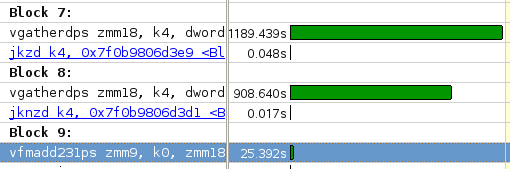
\includegraphics[width=0.49\textwidth]{figures/vtune_naive.png}
    \caption{Vtune profiler in the native kernel.}
    \label{vtune_naive}
\end{figure}

\par{Also figure \ref{Naive} shows that not in all of the \emph{work group} sizes it is possible to execute the kernel in the GPU. 
This is because the GPU run out of resources in those cases\cite{opencl_error} as its possible to see in figure 
\ref{GpuDeviceInfo}(Max \emph{work group} size).}

\par{Reading the listing \ref{naive_kernel}, its possible to see that there is no effort to use caches efficiently, the locality of
    memory access pattern its far from ideal. At the top of this, the gathering of data from memory force to have a high CPI(clock per
    instructions)\footnote{The CPI value of an application or function is an indication of how much latency affected its execution. 
    Higher CPI values mean there was more latency in your system – on average, it took more clockticks for an instruction to retire. 
    Latency in your system can be caused by cache misses, I/O, or other bottlenecks\cite{cpi}.} 
    rate. This is true even in the Xeon and Xeon Phi where both count with an automatic caching system.}

\par{Figure \ref{NaiveComp} shows that GPUs achived the best performance in comparison with the other architectures particularly
    in the case where the \emph{work group} dimension is 1x1024 this is mainly because with 1x1024 the memory access pattern to 
    matrix B its coalesced which means that the GPU can combine several memory accesses into a single transaction.(\emph{deeper..})}

\begin{figure}[!h]
    \centering
    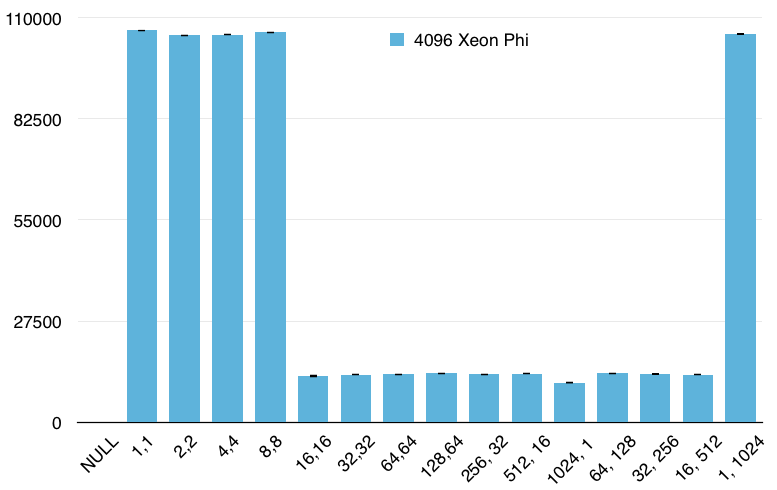
\includegraphics[width=0.49\textwidth]{figures/naive_phi.png}
    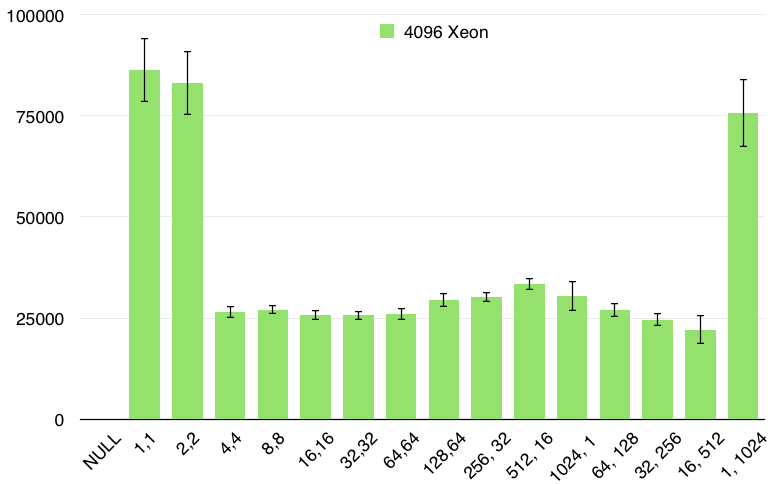
\includegraphics[width=0.49\textwidth]{figures/naive_cpu.png}
    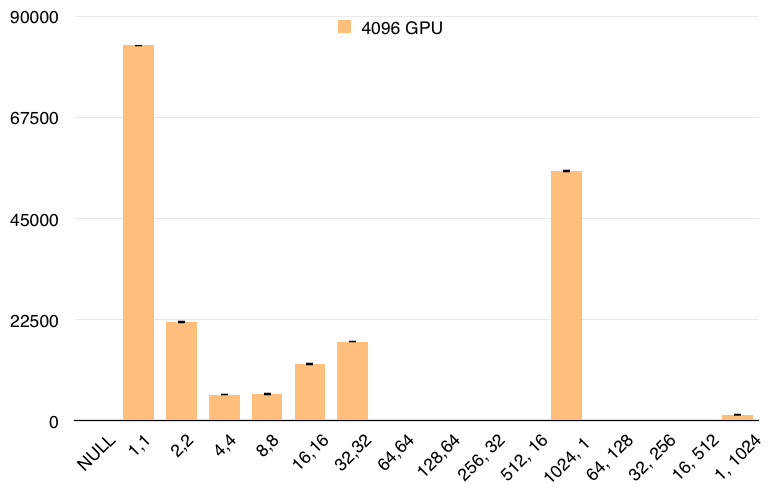
\includegraphics[width=0.49\textwidth]{figures/naive_gpu.png}
    \caption{Naive matrix multiplication in different architectures.}
    \label{Naive}
\end{figure}


